\documentclass{article}

\usepackage{arxiv}

\usepackage[utf8]{inputenc} % allow utf-8 input
\usepackage[T1]{fontenc}    % use 8-bit T1 fonts
\usepackage{lmodern}        % https://github.com/rstudio/rticles/issues/343
\usepackage{hyperref}       % hyperlinks
\usepackage{url}            % simple URL typesetting
\usepackage{booktabs}       % professional-quality tables
\usepackage{amsfonts}       % blackboard math symbols
\usepackage{nicefrac}       % compact symbols for 1/2, etc.
\usepackage{microtype}      % microtypography
\usepackage{graphicx}

\title{Bayesian Small Area Estimation of Under-Five Malaria Prevalence
in West Africa}

\author{
    Godwill Zulu
   \\
    School of Mathematics, Statistics and Applied Mathematics,
University of Galway, Galway, Ireland \\
   \\
  \texttt{\href{mailto:g.zulu1@universityofgalway.ie}{\nolinkurl{g.zulu1@universityofgalway.ie}}} \\
   \And
    Steward Hagen
   \\
    School of Mathematics, Statistics and Applied Mathematics,
University of Galway, Galway, Ireland \\
   \\
  \texttt{} \\
  }


% tightlist command for lists without linebreak
\providecommand{\tightlist}{%
  \setlength{\itemsep}{0pt}\setlength{\parskip}{0pt}}


% Pandoc citation processing
%From Pandoc 3.1.8
% definitions for citeproc citations
\NewDocumentCommand\citeproctext{}{}
\NewDocumentCommand\citeproc{mm}{%
  \begingroup\def\citeproctext{#2}\cite{#1}\endgroup}
\makeatletter
 % allow citations to break across lines
 \let\@cite@ofmt\@firstofone
 % avoid brackets around text for \cite:
 \def\@biblabel#1{}
 \def\@cite#1#2{{#1\if@tempswa , #2\fi}}
\makeatother
\newlength{\cslhangindent}
\setlength{\cslhangindent}{1.5em}
\newlength{\csllabelwidth}
\setlength{\csllabelwidth}{3em}
\newenvironment{CSLReferences}[2] % #1 hanging-indent, #2 entry-spacing
 {\begin{list}{}{%
  \setlength{\itemindent}{0pt}
  \setlength{\leftmargin}{0pt}
  \setlength{\parsep}{0pt}
  % turn on hanging indent if param 1 is 1
  \ifodd #1
   \setlength{\leftmargin}{\cslhangindent}
   \setlength{\itemindent}{-1\cslhangindent}
  \fi
  % set entry spacing
  \setlength{\itemsep}{#2\baselineskip}}}
 {\end{list}}
\usepackage{calc}
\newcommand{\CSLBlock}[1]{#1\hfill\break}
\newcommand{\CSLLeftMargin}[1]{\parbox[t]{\csllabelwidth}{#1}}
\newcommand{\CSLRightInline}[1]{\parbox[t]{\linewidth - \csllabelwidth}{#1}\break}
\newcommand{\CSLIndent}[1]{\hspace{\cslhangindent}#1}

\usepackage{amsmath}
\usepackage{amssymb}
\usepackage{bm}
\usepackage{booktabs}
\usepackage{longtable}
\usepackage{float}
\usepackage{booktabs}
\usepackage{longtable}
\usepackage{array}
\usepackage{multirow}
\usepackage{wrapfig}
\usepackage{float}
\usepackage{colortbl}
\usepackage{pdflscape}
\usepackage{tabu}
\usepackage{threeparttable}
\usepackage{threeparttablex}
\usepackage[normalem]{ulem}
\usepackage{makecell}
\usepackage{xcolor}
\begin{document}
\maketitle


\begin{abstract}
District-level estimates of malaria prevalence are needed to target
control interventions, but the household surveys that supply them cover
only a fraction of districts and yield unstable estimates wherever few
clusters are sampled. We address both problems with a Bayesian
spatio-temporal small area estimation framework applied to under-five
malaria prevalence across Ghana, Burkina Faso and Côte d'Ivoire, using
two rounds of Demographic and Health Survey biomarker data covering 724
districts. Design-based Hájek prevalence estimates and their
Taylor-linearised sampling variances enter an area-level Fay-Herriot
model equipped with a scaled BYM2 spatial prior and a Knorr-Held Type I
space-time interaction. We progress through four specifications: a
cross-sectional Ghana baseline, separate country-level space-time
models, a single-round pooled three-country model that establishes
cross-border smoothing on temporally aligned data, and a pooled
space-time model that adds the temporal dimension and is benchmarked
against the single-round model to confirm the cross-border structure is
not an artefact of joining surveys from different years. The estimated
national trajectories differ sharply across the three countries: Ghana
and Burkina Faso show large declines between rounds (odds ratios of
roughly 0.32 and 0.08), while Côte d'Ivoire shows an increase (odds
ratio near 2.1). Urbanisation, proxied by nighttime lights, is the most
consistent protective covariate across all three countries. Pooling
raises the structured share of spatial variation from roughly one half
to four fifths and rescues many noisy districts into a usable
reliability range. The framework fills unobserved districts, stabilises
noisy direct estimates and flags districts that diverge from their
national trend, providing a defensible regional evidence base for
subnational malaria planning.
\end{abstract}

\keywords{
    small area estimation
   \and
    Bayesian hierarchical models
   \and
    BYM2
   \and
    Fay-Herriot
   \and
    malaria
   \and
    spatio-temporal modelling
   \and
    West Africa
  }

\section{Introduction}\label{introduction}

Malaria continues to impose a heavy burden of childhood illness and
death across sub-Saharan Africa, and the countries of West Africa bear a
disproportionate share of it (World Health Organization 2023). The
interventions that have driven the regional decline of the past two
decades insecticide-treated nets, seasonal malaria chemoprevention,
intermittent preventive treatment in pregnancy and indoor residual
spraying are planned, financed and delivered through district health
systems. Decisions about where to send nets, where to run a
chemoprevention campaign and where to investigate a resurgence are
therefore made at the district scale. The evidence used to make them,
however, is usually summarised at the regional or national level, which
hides the district-to-district variation that targeting depends on.

Two features of household survey data stand in the way of direct
district-level estimation. The first is incomplete spatial coverage. The
Demographic and Health Surveys (DHS) provide the most reliable
population-based measurements of malaria infection in children through
rapid diagnostic testing (Florey 2014; {Croft et al.} 2018), but survey
clusters are placed in only a subset of districts within each country.
In the surveys analysed here, between roughly forty and seventy per cent
of districts contain at least one cluster in any given round, leaving
the remainder with no direct measurement at all. The second feature is
sampling instability. Even where a district is sampled, an estimate
built from a handful of clusters carries a wide design-based standard
error, so that the apparent geography of risk can be dominated by survey
noise rather than by any real signal.

Small area estimation responds to both problems by borrowing strength
(Rao and Molina 2015; Wakefield et al. 2020). The area-level model of
Fay and Herriot treats each district's direct estimate as a noisy
reading of an unobserved true prevalence, and separates the sampling
error which is treated as known from the survey design from the residual
variation that the model is free to learn. A spatial prior lets
neighbouring districts inform one another, a temporal component lets
survey rounds inform one another, and auxiliary covariates let districts
that resemble each other in their environmental and socio-economic
profile share information as well. The result is a complete prevalence
surface with calibrated uncertainty, including for districts that were
never sampled.

This report develops such a framework and applies it jointly to Ghana,
Burkina Faso and Côte d'Ivoire. The three countries are geographically
contiguous, share the dominant \emph{Anopheles} vector species and the
West African monsoon that drives seasonal transmission, and have pursued
overlapping but not identical intervention programmes. They are also a
useful test of multi-country modelling because their recent prevalence
trajectories diverge: as the results below show, two of the three have
declined sharply between survey rounds while the third has worsened. We
ask four questions. Can a spatial model with a BYM2 prior produce
reliable district estimates, including for unobserved districts, from
DHS data and standard covariates? How has prevalence moved between
rounds in each country, and which districts depart from the national
trend? Which covariates drive spatial variation, and do their effects
differ across countries? And does a pooled model that smooths across
national borders and partially pools covariate effects improve on
separate country models while remaining defensible when the survey
calendars do not align?

The remainder of the report is organised around the data pipeline and a
sequence of four models. Section \ref{sec:data} describes the surveys,
the adjacency structure and the covariate panel, and sets out how the
direct estimates and their sampling variances are computed. Section
\ref{sec:methods} states the common modelling machinery. The four models
then build in sequence: a cross-sectional baseline that isolates the
spatial structure (Section \ref{sec:m1}), country-level space-time
models that recover each national trajectory (Section \ref{sec:m2}), a
single-round pooled model that establishes cross-border smoothing on
temporally aligned data (Section \ref{sec:m3}), and a pooled space-time
model that adds the temporal dimension and is checked against the
single-round model (Section \ref{sec:m4}). Section \ref{sec:validation}
sets out the planned external validation against the Malaria Atlas
Project and the sensitivity analyses. Section \ref{sec:discussion} draws
the findings together, Section \ref{sec:limitations} states the
limitations, and Section \ref{sec:conclusion} concludes.

\section{Data and Direct Estimation}\label{sec:data}

\subsection{Survey data}\label{survey-data}

The data come from the DHS programme, which fields nationally
representative household surveys using a stratified two-stage cluster
design ({Croft et al.} 2018). Enumeration areas are selected within
strata defined by region and urban or rural residence, and households
are selected within each sampled cluster. Children aged six to
fifty-nine months are tested for malaria infection by rapid diagnostic
test, the field standard since around 2010 (Florey 2014). Cluster
coordinates are displaced by up to five kilometres in urban areas and
ten in rural areas to protect respondent confidentiality. We use the
household member recode file for the individual-level biomarker and the
cluster GPS shapefile for spatial referencing. Two rounds are used per
country: Ghana 2014 and 2022, Burkina Faso 2010 and 2021, and Côte
d'Ivoire 2012 and 2021 (Table \ref{tab:surveys}).

\begin{longtable}[t]{lllr}
\caption{\label{tab:surveys}\label{tab:surveys}DHS survey rounds and district counts by country.}\\
\toprule
Country & Round 1 & Round 2 & Districts\\
\midrule
Burkina Faso & DHS 2010 & DHS 2021 & 351\\
Côte d'Ivoire & DHS 2012 & DHS 2021 & 113\\
Ghana & DHS 2014 & DHS 2022 & 260\\
\bottomrule
\end{longtable}

\subsection{Administrative boundaries and
adjacency}\label{administrative-boundaries-and-adjacency}

District boundaries were taken from the Global Administrative Areas
database, at the second administrative level for Ghana and the third for
Burkina Faso and Côte d'Ivoire, which correspond to the units at which
the national malaria programmes operate. The combined panel contains 724
districts (260, 351 and 113 respectively). Adjacency was defined by
queen contiguity using \texttt{spdep} (Bivand et al. 2013), and any
districts left without neighbours were reconnected using a small snap
tolerance so that the intrinsic conditional autoregressive prior remains
proper (Freni-Sterrantino et al. 2018). The single-country graphs
contain 709, 973 and 296 edges; the combined 724-district graph contains
2,056 edges, of which 78 cross a national border (Table
\ref{tab:spatial}). These cross-border edges are what allow districts
near a frontier to borrow information from their neighbours in the
adjacent country.

\begin{longtable}[t]{lrrr}
\caption{\label{tab:spatial}\label{tab:spatial}Adjacency graph sizes and BYM2 scaling factors. The combined graph adds 78 cross-border edges.}\\
\toprule
Country & Districts & Edges & Scaling factor\\
\midrule
Ghana & 260 & 709 & 4.36\\
Burkina Faso & 351 & 973 & 3.36\\
Côte d'Ivoire & 113 & 296 & 9.30\\
Combined & 724 & 2056 & NA\\
\bottomrule
\end{longtable}

\subsection{Covariates}\label{covariates}

Seven covariates were assembled at the district-round level: elevation
(SRTM, population-weighted), rainfall (CHIRPS v2.0, September to
December mean), nighttime lights (NASA Black Marble VIIRS) as a proxy
for urbanisation (Elvidge et al. 2013), temperature (CRU TS v4.09,
September to December mean), travel time to the nearest health facility
(Weiss et al., population-weighted) ({Weiss et al.} 2019), log
population density (WorldPop), and a multidimensional poverty headcount
(OPHI MPI and national census). Each covariate was standardised within
country, so that coefficients describe the effect of a
one-standard-deviation change, a single weakly informative prior applies
across all of them, and the Hamiltonian Monte Carlo sampler explores a
better-conditioned posterior. All retained pairwise correlations stayed
below the conventional threshold of 0.7 ({Dormann et al.} 2013);
nighttime lights and log population density, though related, were both
kept because they capture distinct aspects of settlement.

\subsection{Direct estimates and sampling
variances}\label{direct-estimates-and-sampling-variances}

For each observed district \(i\) in round \(t\) we formed a design-based
prevalence estimate using the Hájek ratio (Hájek 1971), \begin{equation}
\hat{p}_{it}^{w} = \frac{\sum_k d_k\, z_k}{\sum_k d_k},
\end{equation} where \(z_k\) is the rapid-test result for child \(k\)
and \(d_k\) the survey weight. Standard errors were obtained by
Taylor-series linearisation (Binder 1983) using the \texttt{survey}
package (Lumley 2010), with the stratified two-stage design carried
through the variance calculation. To fit the Gaussian Fay-Herriot
likelihood we worked on the logit scale, transforming the standard error
by the delta method, \begin{equation}
y_{it} = \mathrm{logit}\!\left(\hat{p}_{it}^{w}\right),
\qquad
\widehat{\mathrm{SE}}(y_{it}) =
\frac{\widehat{\mathrm{SE}}(\hat{p}_{it}^{w})}
     {\hat{p}_{it}^{w}\,(1 - \hat{p}_{it}^{w})}.
\end{equation} For numerical stability, prevalences were bounded to
\([0.02, 0.98]\) and logit-scale standard errors to \([0.1, 2.0]\)
before entering the model. Coverage varied by country and round: of 260
Ghana districts, 153 were observed in 2014 and 124 in 2022; of 351
Burkina Faso districts, 232 in 2010 and 153 in 2021; and of 113 Côte
d'Ivoire districts, 80 in 2012 and 103 in 2021.

\section{Common Methodology}\label{sec:methods}

All four models share a Fay-Herriot likelihood, a scaled BYM2 spatial
prior and a common set of penalised-complexity priors. We state these
once here; each model section then adds only what is specific to it.

\subsection{Fay-Herriot likelihood}\label{fay-herriot-likelihood}

The direct estimate is modelled as a noisy observation of a latent logit
prevalence, \begin{equation}
y_{it} \sim \mathcal{N}\!\left(\theta_{it},\, \psi_{it}^2\right),
\end{equation} with the sampling variance \(\psi_{it}^2\) treated as
known (Wakefield et al. 2020). This is the standard area-level
simplification; its consequences for districts with very few clusters
are returned to in Section \ref{sec:limitations}.

\subsection{BYM2 spatial prior}\label{bym2-spatial-prior}

Every model places a scaled BYM2 prior (Riebler et al. 2016) on the
district-level spatial effect, written in non-centred form,
\begin{equation}
b_i = \sigma_b\!\left(\sqrt{1-\phi}\, v_i + \sqrt{\phi/s}\, u_i\right),
\qquad
v_i \sim \mathcal{N}(0,1),
\qquad
u_i \sim \mathrm{ICAR}(W).
\end{equation} Here \(v_i\) is an unstructured component, \(u_i\) a
spatially structured intrinsic conditional autoregressive component,
\(\sigma_b\) the marginal standard deviation of the combined effect, and
\(\phi \in (0,1)\) the share of variance that is spatially structured.
The scaling constant \(s\), computed from the graph, makes \(\phi\)
comparable across the different adjacency structures, which the original
BYM model could not guarantee (Besag et al. 1991). The non-centred form
avoids the funnel geometry that otherwise couples \(\sigma_b\) to the
random effects.

\subsection{Priors}\label{priors}

The intercept used a weakly informative \(\mathcal{N}(-1.85, 1)\) prior,
centred near the logit of a moderate prevalence. The spatial standard
deviation used an exponential penalised-complexity prior approximating
\(P(\sigma_b > 1) = 0.01\) (Simpson et al. 2017), the mixing parameter a
\(\mathrm{Beta}(3,2)\) prior with a mild preference for structured over
unstructured variation, and standardised covariate coefficients a shared
\(\mathcal{N}(0,1)\) prior. The space-time interaction standard
deviation and the between-country slope standard deviations both used
\(\mathrm{Exp}(2)\) penalised-complexity priors.

\subsection{Computation}\label{computation}

All models were fitted in Stan (Stan Development Team 2024) through the
\texttt{cmdstanr} interface, using the No-U-Turn Sampler with
non-centred parameterisations throughout. Each model ran four chains
with 1,500 warmup and 2,000 sampling iterations. The cross-sectional and
country-level space-time models used \texttt{adapt\_delta} 0.99 and a
maximum tree depth of 14; the larger pooled models used 0.97 and 13.
Convergence was judged by the \(\hat{R}\) statistic, bulk and tail
effective sample sizes (Vehtari et al. 2017) and inspection of trace,
rank and pairs plots; across the models reported here \(\hat{R}\) stayed
at or below about 1.02 with no divergent transitions. Competing
specifications were compared by approximate leave-one-out
cross-validation (Vehtari et al. 2017).

\section{Model 1: Cross-Sectional Ghana Baseline}\label{sec:m1}

\subsection{Specification}\label{specification}

The baseline model isolates the spatial component by restricting
attention to a single country and round, Ghana in 2022, \begin{equation}
\theta_i = \mu + b_i + \mathbf{x}_i^{\top}\bm{\beta},
\end{equation} with \(b_i\) the scaled BYM2 effect defined in the common
methodology. The attraction of the BYM2 parameterisation is that it does
not force a choice between an unstructured and a structured spatial
model; it contains both as limiting cases and lets the data decide the
balance between them. Recall that \begin{equation}
b_i = \sigma_b\!\left(\sqrt{1-\phi}\, v_i + \sqrt{\phi/s}\, u_i\right),
\end{equation} where \(v_i\) is the unstructured (independent) component
and \(u_i\) the structured ICAR component. Setting the mixing parameter
\(\phi = 0\) removes the structured part entirely and the model
collapses to a purely independent (IID) specification in which each
district is shrunk toward the national mean on its own; setting
\(\phi = 1\) removes the unstructured part and the model becomes a pure
ICAR in which every district is informed wholly by its neighbours. For
intermediate values, \(\phi\) is interpretable as the proportion of the
residual spatial variance that is geographically structured, so the
single parameter both decides whether IID or ICAR behaviour dominates
and quantifies the split between them. To confirm that this flexibility
is warranted rather than assumed, we fit the two limiting cases
explicitly IID (\(\phi\) fixed at 0) and ICAR (\(\phi\) fixed at 1) and
compare all three by leave-one-out cross-validation.

\subsection{Results}\label{results}

The cross-validation is decisive about what to exclude and permissive
about what to keep (Figure \ref{fig:m1loo}, Table \ref{tab:m1loo}). The
pure ICAR model is clearly the worst of the three, trailing the best by
about seven units of expected log predictive density with a standard
error that does not cover zero; forcing every district to be explained
entirely by its neighbours is too rigid for Ghana's data. The BYM2 and
IID models, by contrast, are statistically indistinguishable, separated
by less than one predictive unit, which tells us that a large share of
the district-level variation in a single cross-section is idiosyncratic
rather than smoothly geographic. The BYM2 posterior makes the same point
from the inside: it places the structured share at
\(\phi \approx 0.44\), so the data themselves attribute roughly half of
the residual spatial variance to geography and half to district-specific
noise.

We adopt the BYM2 prior as the working spatial structure for this and
every subsequent model, for two reasons that the cross-validation makes
concrete. First, BYM2 is never worse than the better of its two limiting
cases here, because it can reproduce either by moving \(\phi\); choosing
it costs nothing in predictive terms relative to IID while retaining the
ability to express structure where structure exists. Second, and
decisively for an estimation task whose purpose is to fill unobserved
districts, only the structured component allows an unsampled district to
borrow from its neighbours. A pure IID model would shrink every
unobserved district to the same national mean and so could not produce a
spatially coherent surface, which is precisely what subnational
targeting requires. Letting \(\phi\) be estimated rather than fixed
means each later model the country-level space-time models and the two
pooled models inherits a spatial prior that adapts the IID-to-ICAR
balance to its own data rather than committing to one extreme in
advance. The BYM2 fit for Ghana 2022 gives a national intercept of
\(-1.82\) on the logit scale, a marginal spatial standard deviation of
\(0.88\), and an implied national prevalence near 14 per cent.

\begin{figure}[H]

{\centering 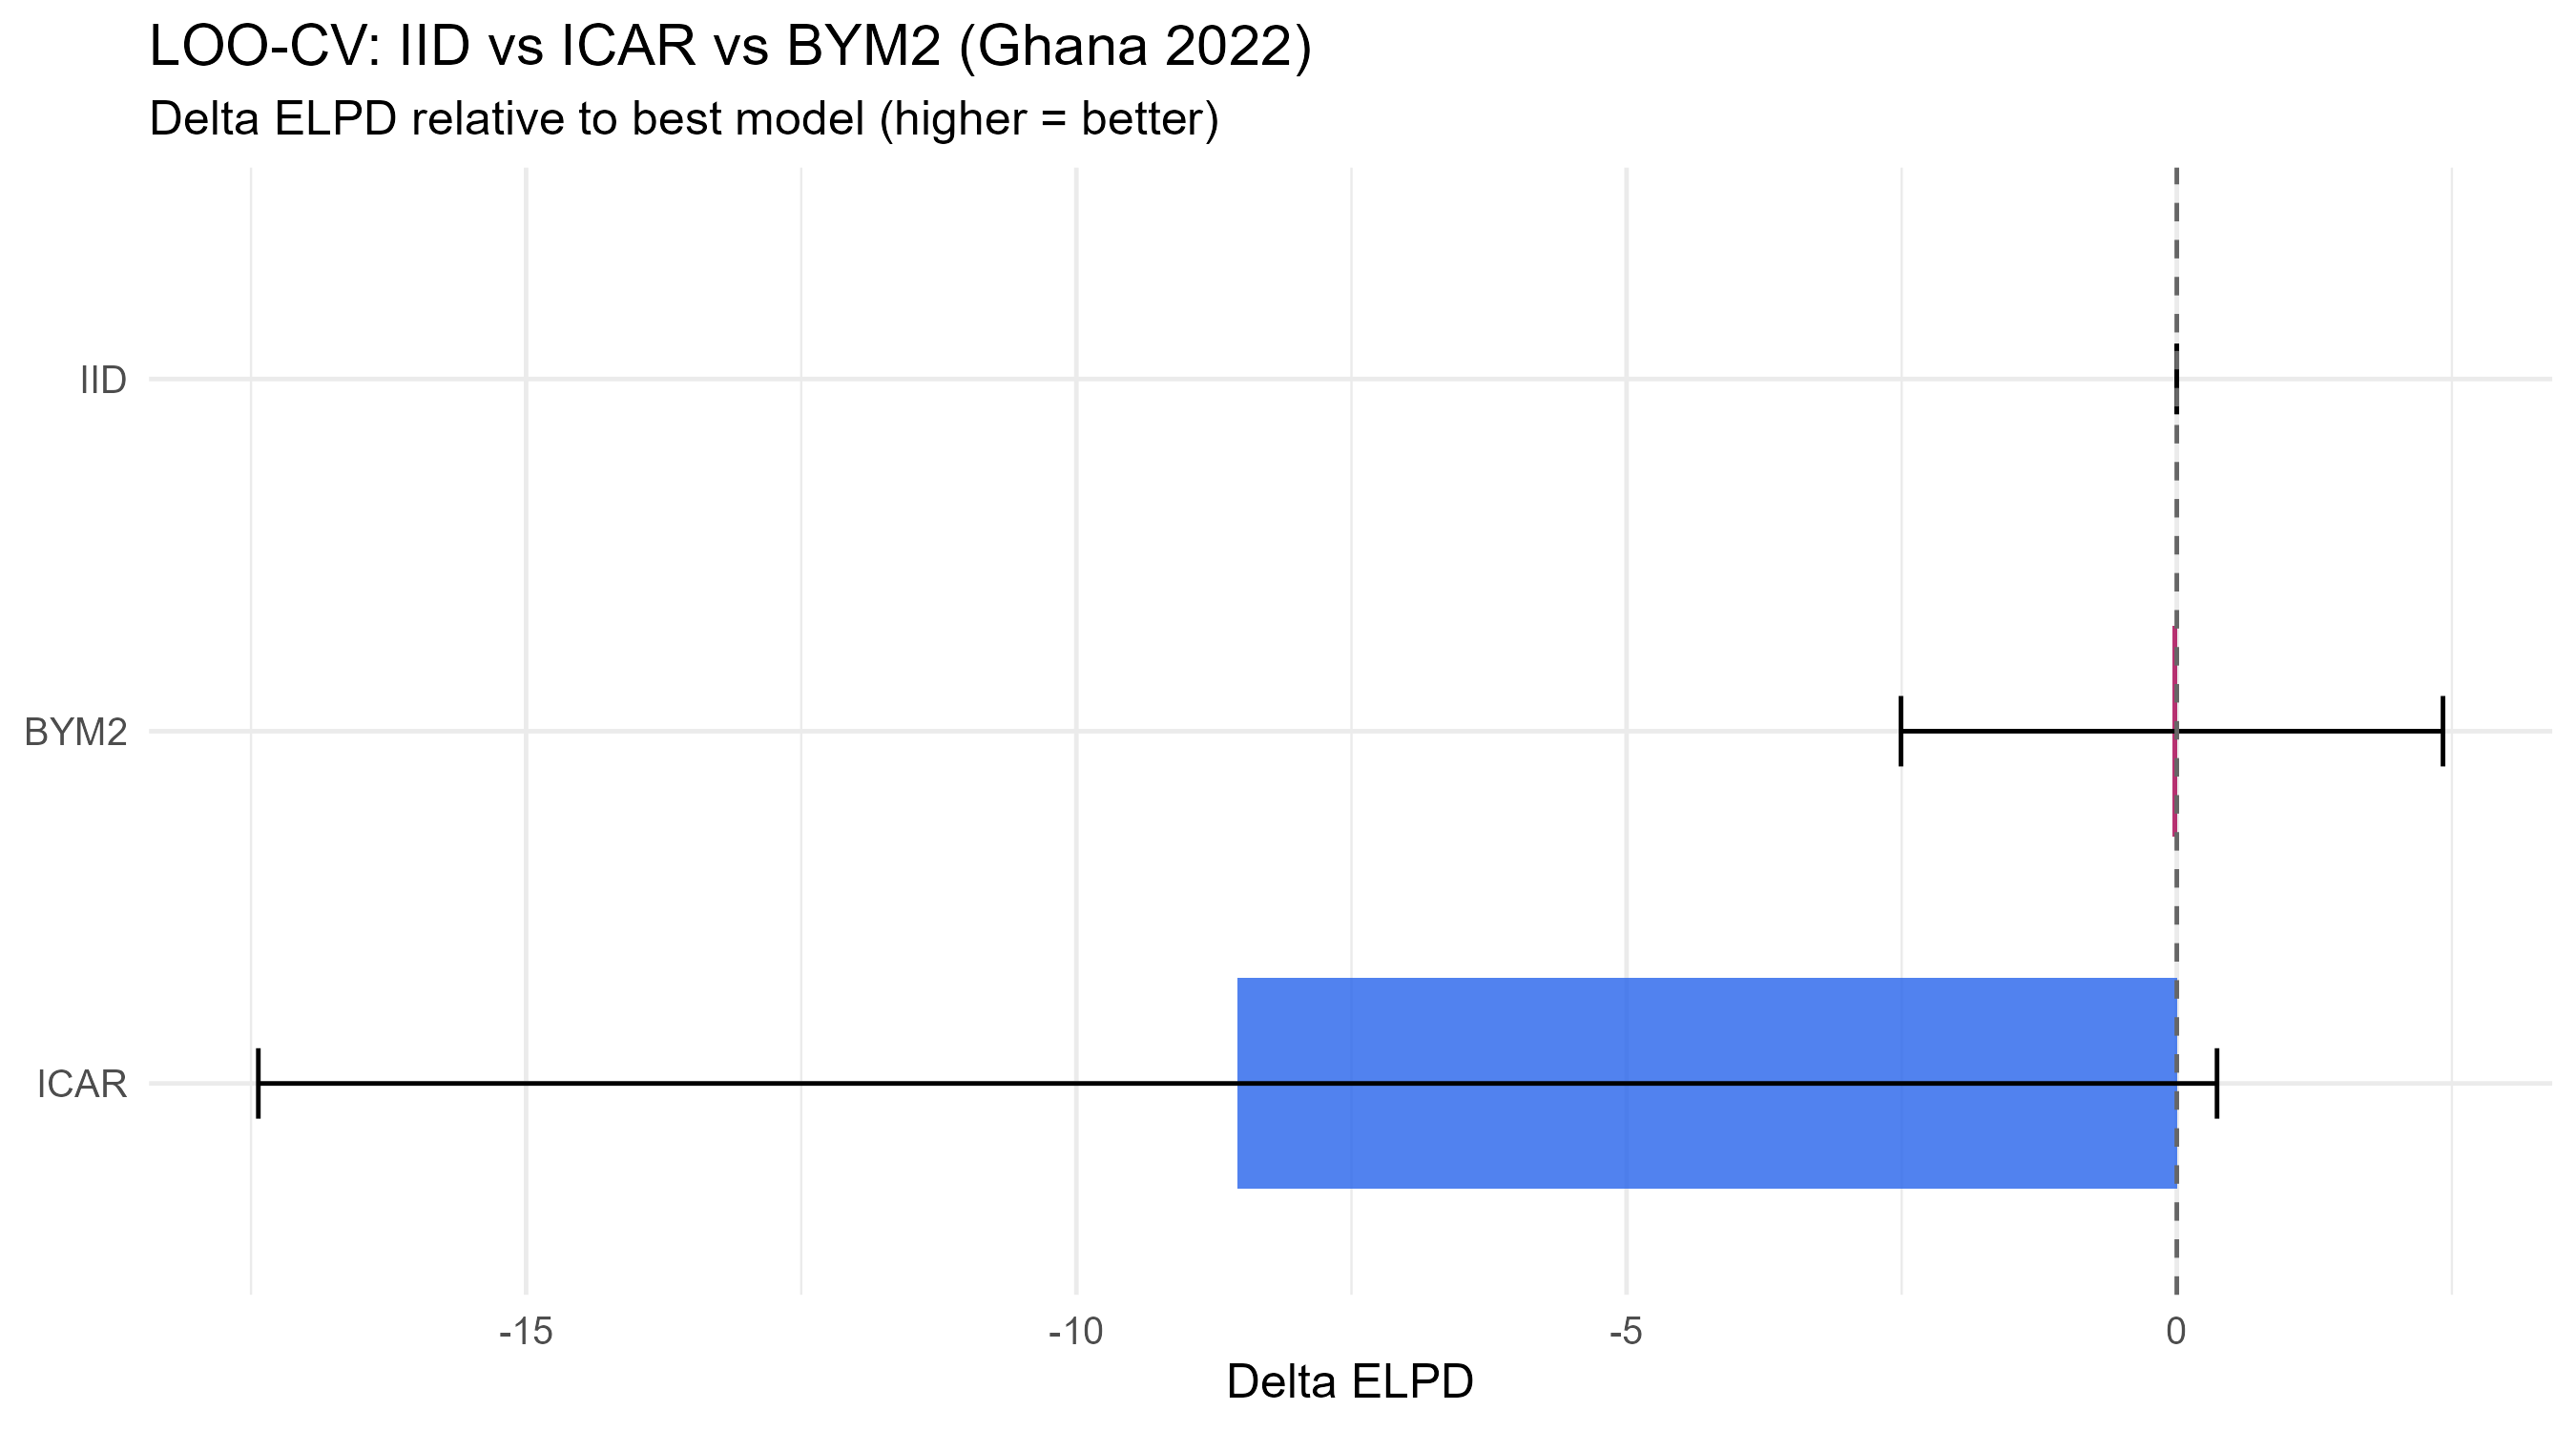
\includegraphics[width=0.85\linewidth]{output/figures/loo_cv_comparison} 

}

\caption{\label{fig:m1loo}Leave-one-out cross-validation for the Ghana 2022 cross-section: change in expected log predictive density relative to the best model, with standard errors. The pure ICAR model is clearly worse; BYM2 and IID are within noise of each other, so BYM2 is retained because it spans both and supports spatial borrowing.}\label{fig:m1loo-fig}
\end{figure}

\begin{longtable}[t]{lllr}
\caption{\label{tab:m1loo}\label{tab:m1loo}Ghana 2022 cross-section: leave-one-out comparison. BYM2 and the unstructured model are within noise of each other; the pure ICAR model is clearly worse.}\\
\toprule
Model & ELPD diff & SE diff & p\_loo\\
\midrule
BYM2 & 0.0 & 0.0 & 68.8\\
IID & -0.3 & 1.3 & 69.3\\
ICAR & -7.3 & 3.8 & 72.8\\
\bottomrule
\end{longtable}

The baseline confirms that the BYM2 machinery fills the unobserved
districts and produces a coherent surface, but it can say nothing about
change over time. The next model adds the temporal dimension.

\section{Model 2: Country-Level Space-Time Models}\label{sec:m2}

\subsection{Specification}\label{specification-1}

Fitting each country separately, the latent prevalence gains a national
temporal shift and an unstructured space-time interaction,
\begin{equation}
\theta_{it} = \mu^{(c)} + b_i^{(c)} + \delta_t^{(c)} + \gamma_{it}^{(c)}
              + \mathbf{x}_{it}^{\top}\bm{\beta}^{(c)},
\qquad
\gamma_{it}^{(c)} \sim \mathcal{N}(0, \sigma_\gamma^2).
\end{equation} With only two rounds, the Knorr-Held Type I interaction
is the only identifiable choice: a temporally structured prior over two
points collapses to a single increment, and spatially structured
interactions are not separable from the main spatial effect at this
length of series (Knorr-Held 2000; Goicoa et al. 2018). The first round
is set as the reference (\(\delta_1 = 0\)) and the second estimated
freely.

\subsection{Results}\label{results-1}

The three countries tell strikingly different stories (Table
\ref{tab:m2}). In Ghana, the temporal shift is \(\delta_2 = -1.14\),
corresponding to a fall in modelled national prevalence from about 30.5
to 12.3 per cent. In Burkina Faso the decline is far steeper, with
\(\delta_2 =
-2.52\) and prevalence dropping from roughly 71.2 to 16.8 per cent. Côte
d'Ivoire moves in the opposite direction: \(\delta_2 = +0.78\), with
prevalence rising from about 17.4 to 31.3 per cent. The contrast between
two countries in rapid retreat and a third moving against the regional
tide is the central empirical finding, and the next sections show it to
be robust to how the data are pooled.

The spatial parameters are also informative. The structured share
\(\phi\) ranges from 0.47 in Ghana through 0.59 in Côte d'Ivoire to 0.64
in Burkina Faso, so that between a half and two thirds of the
unexplained variation is geographic in each country. Burkina Faso
carries the largest marginal spatial standard deviation at 1.04,
consistent with its pronounced north-to-south transmission gradient. The
interaction standard deviation sits near 0.5 in all three countries,
indicating that individual districts do depart from the national trend
by a meaningful amount; the term \(\gamma_{it}\) records exactly which
ones.

\begin{longtable}[t]{llll}
\caption{\label{tab:m2}\label{tab:m2}Country-level space-time posterior summaries. Ghana and Burkina Faso decline sharply between rounds; Côte d'Ivoire rises.}\\
\toprule
Parameter & Ghana & Burkina Faso & Côte d'Ivoire\\
\midrule
\$\textbackslash{}delta\_2\$ (time shift) & -1.14 & -2.52 & +0.78\\
Round 1 prevalence & 30.5\textbackslash{}\% & 71.2\textbackslash{}\% & 17.4\textbackslash{}\%\\
Round 2 prevalence & 12.3\textbackslash{}\% & 16.8\textbackslash{}\% & 31.3\textbackslash{}\%\\
\$\textbackslash{}sigma\_b\$ & 0.72 & 1.04 & 0.82\\
\$\textbackslash{}phi\$ & 0.47 & 0.64 & 0.59\\
\addlinespace
\$\textbackslash{}sigma\_\textbackslash{}gamma\$ & 0.52 & 0.52 & 0.48\\
\bottomrule
\end{longtable}

Mapping the interaction term for Ghana identifies districts that have
diverged from the national decline: a band of districts whose 95 per
cent intervals exclude zero have fallen behind the national pace of
improvement, while others have outpaced it. These are the districts a
programme manager would single out for investigation, since they are not
explained by the country-wide trend, by their neighbours or by the
measured covariates.

What the country-level models cannot do is share information across
borders or pull a regional consensus from the covariate effects. Côte
d'Ivoire in particular, with the fewest districts, would benefit from
borrowing. The pooled models that follow address this, beginning with
the temporally aligned single-round model.

\section{Model 3: Single-Round Pooled Three-Country Model}\label{sec:m3}

\subsection{Motivation}\label{motivation}

The country-level models treat each country as a spatial island, yet the
three countries share borders, vector species and the monsoon that
drives transmission. The natural next step is to pool them on a single
adjacency graph so that districts near a frontier can borrow from their
neighbours across the national line. Pooling across two survey rounds at
once, however, raises a question about the spatial smoother: the Round 1
surveys span four calendar years (Burkina Faso 2010, Côte d'Ivoire 2012,
Ghana 2014), and a graph that smooths residuals across borders in that
earlier round would be mixing space with time over a period in which
intervention coverage and rainfall changed appreciably. It is not
obvious that cross-border adjacency is meaningful when the surfaces
being joined are years apart.

We therefore establish the cross-border case first on its cleanest
footing, using only the contemporaneous second round (Burkina Faso 2021,
Côte d'Ivoire 2021, Ghana 2022), which falls within a single year. With
a single round the temporal shift and the space-time interaction
disappear, and the model reduces to a pure spatial BYM2 over all 724
districts with hierarchical covariate slopes. The cross-border smoothing
now operates on genuinely simultaneous surfaces, so the spatial
borrowing cannot be confounded with temporal change. This single-round
pooled model is the methodologically conservative cross-border
specification; the temporal extension that follows in Section
\ref{sec:m4} is then read against it.

\subsection{Specification}\label{specification-2}

For each observed Round 2 district \(i\), \begin{equation}
\theta_i = \mu + \alpha_{c[i]} + b_i + \mathbf{x}_i^{\top}\bm{\beta}_{c[i]},
\qquad
\beta_{ck} \sim \mathcal{N}(\bar{\beta}_k, \tau_k^2).
\end{equation} The country deviations \(\alpha_c\) are constrained to
sum to zero so that they are identified against the grand intercept
\(\mu\), the spatial effect \(b_i\) is the BYM2 field on the combined
724-district graph including its 78 cross-border edges, and the
covariate slopes for each country are drawn around a shared regional
mean \(\bar{\beta}_k\) with between-country spread \(\tau_k\). The
closest published cross-border application used a comparable two-year
alignment window (Saldarriaga 2020); the single-year window here is
tighter still. Priors and the adjacency graph are exactly those of the
common methodology, so nothing in the comparison with the temporal model
that follows is driven by a change of specification.

\subsection{Results}\label{results-2}

\section{Model 4: Pooled Three-Country Space-Time Model}\label{sec:m4}

\subsection{Motivation}\label{motivation-1}

The single-round pooled model of Section \ref{sec:m3} establishes the
cross-border spatial structure on temporally aligned data but discards
half the evidence: it says nothing about change between rounds. The full
space-time model restores the temporal dimension, fitting all 724
districts and both rounds jointly with country intercepts,
country-specific temporal shifts and hierarchical covariate slopes. In
doing so it must confront the concern raised earlier that the
cross-border edges in the earlier round smooth across surfaces several
years apart. The model's defence is structural: the country-specific
shifts \(\delta_{c,t}\) absorb each country's own level and trend before
the shared spatial field operates on the residuals, so the field is
smoothing deviations from each national trajectory rather than raw
prevalence across time. Whether that defence holds is then checked
empirically by comparing this model's spatial parameters and covariate
means against the temporally aligned single-round model of Section
\ref{sec:m3}.

\subsection{Specification}\label{specification-3}

\begin{equation}
\theta_{it} = \mu + \alpha_{c[i]} + b_i + \delta_{c[i],t} + \gamma_{it}
              + \mathbf{x}_{it}^{\top}\bm{\beta}_{c[i]},
\qquad
\beta_{ck} \sim \mathcal{N}(\bar{\beta}_k, \tau_k^2).
\end{equation} The country deviations sum to zero, the temporal shifts
\(\delta_{c,t}\) free each national trajectory with the first round as
reference, and \(\gamma_{it}\) is the Knorr-Held Type I interaction. The
spatial effect operates on the same combined graph as Model 4, so the
only additions relative to that model are the temporal terms.

\subsection{Results}\label{results-3}

\begin{longtable}[t]{lll}
\caption{\label{tab:m4-pooled-st}\label{tab:m4}Pooled space-time model: country-specific temporal shifts and implied between-round odds ratios. The shared spatial field has $\sigma_b = 0.65$ and $\phi = 0.83$.}\\
\toprule
Country & \$\textbackslash{}delta\_2\$ & Odds ratio\\
\midrule
Ghana & -1.13 & 0.32\\
Côte d'Ivoire & +0.74 & 2.13\\
Burkina Faso & -2.53 & 0.08\\
\bottomrule
\end{longtable}

\section{External Validation and Sensitivity
Analyses}\label{sec:validation}

The estimates presented above are internally coherent and well behaved
under the model's own diagnostics, but a full assessment requires
checking them against an independent source and probing their
sensitivity to the modelling choices. To be done\ldots{}

\subsection{Validation against the Malaria Atlas
Project}\label{validation-against-the-malaria-atlas-project}

The Malaria Atlas Project publishes model-based geostatistical surfaces
of \emph{Plasmodium falciparum} parasite-rate for sub-Saharan Africa,
built from a different evidence base and a different modelling tradition
than the area-level approach used here ({Bhatt et al.} 2015; {Weiss et
al.} 2019). To be done\ldots..

\subsection{Sensitivity analyses}\label{sensitivity-analyses}

\section{Discussion}\label{sec:discussion}

\section{Limitations and Future Work}\label{sec:limitations}

\section{Conclusion}\label{sec:conclusion}

\section*{Acknowledgements}\label{acknowledgements}
\addcontentsline{toc}{section}{Acknowledgements}

We thank Dr Nicola Fitz-Simon for supervision and the DHS Program for
access to the survey data

\section*{References}\label{references}
\addcontentsline{toc}{section}{References}

\protect\phantomsection\label{refs}
\begin{CSLReferences}{1}{1}
\bibitem[\citeproctext]{ref-besag1991}
Besag, Julian, Jeremy York, and Annie Mollié. 1991. {``Bayesian Image
Restoration, with Two Applications in Spatial Statistics.''}
\emph{Annals of the Institute of Statistical Mathematics} 43 (1): 1--20.

\bibitem[\citeproctext]{ref-bhatt2015}
{Bhatt, Samir, D. J. Weiss, E. Cameron, et al.} 2015. {``The Effect of
Malaria Control on Plasmodium Falciparum in Africa Between 2000 and
2015.''} \emph{Nature} 526 (7572): 207--11.

\bibitem[\citeproctext]{ref-binder1983}
Binder, David A. 1983. {``On the Variances of Asymptotically Normal
Estimators from Complex Surveys.''} \emph{International Statistical
Review} 51 (3): 279--92.

\bibitem[\citeproctext]{ref-bivand2013}
Bivand, Roger S., Edzer Pebesma, and Virgilio Gómez-Rubio. 2013.
\emph{Applied Spatial Data Analysis with r}. 2nd ed. Springer.

\bibitem[\citeproctext]{ref-croft2018}
{Croft, Trevor N., Aileen M. J. Marshall, Courtney K. Allen, et al.}
2018. \emph{Guide to DHS Statistics}. ICF.

\bibitem[\citeproctext]{ref-dormann2013}
{Dormann, Carsten F., Jane Elith, Sven Bacher, et al.} 2013.
{``Collinearity: A Review of Methods to Deal with It and a Simulation
Study Evaluating Their Performance.''} \emph{Ecography} 36 (1): 27--46.

\bibitem[\citeproctext]{ref-elvidge2014}
Elvidge, Christopher D., Kimberly E. Baugh, Mikhail Zhizhin, and
Feng-Chi Hsu. 2013. {``Why VIIRS Data Are Superior to DMSP for Mapping
Nighttime Lights.''} \emph{Proceedings of the Asia-Pacific Advanced
Network} 35: 62--69.

\bibitem[\citeproctext]{ref-florey2014}
Florey, Lia. 2014. \emph{Measures of Malaria Parasitaemia Prevalence in
National Surveys: Agreement Between Rapid Diagnostic Tests and
Microscopy}. DHS Analytical Studies No. 43. ICF International.

\bibitem[\citeproctext]{ref-freni2018}
Freni-Sterrantino, Anna, Massimo Ventrucci, and Håvard Rue. 2018. {``A
Note on Intrinsic Conditional Autoregressive Models for Disconnected
Graphs.''} \emph{Spatial and Spatio-Temporal Epidemiology} 26: 25--34.

\bibitem[\citeproctext]{ref-goicoa2018}
Goicoa, Tomas, Aritz Adin, María Dolores Ugarte, and James S. Hodges.
2018. {``In Spatio-Temporal Disease Mapping Models, Identifiability
Constraints Affect PQL and INLA Results.''} \emph{Stochastic
Environmental Research and Risk Assessment} 32 (3): 749--70.

\bibitem[\citeproctext]{ref-hajek1971}
Hájek, Jaroslav. 1971. {``Comment on {`an Essay on the Logical
Foundations of Survey Sampling, Part One'}.''} \emph{Foundations of
Statistical Inference} (Toronto), 236.

\bibitem[\citeproctext]{ref-knorrheld2000}
Knorr-Held, Leonhard. 2000. {``Bayesian Modelling of Inseparable
Space-Time Variation in Disease Risk.''} \emph{Statistics in Medicine}
19 (17-18): 2555--67.

\bibitem[\citeproctext]{ref-lumley2010}
Lumley, Thomas. 2010. \emph{Complex Surveys: A Guide to Analysis Using
r}. John Wiley \& Sons.

\bibitem[\citeproctext]{ref-rao2015}
Rao, J. N. K., and Isabel Molina. 2015. \emph{Small Area Estimation}.
2nd ed. John Wiley \& Sons.

\bibitem[\citeproctext]{ref-riebler2016}
Riebler, Andrea, Sigrunn H. Sørbye, Daniel Simpson, and Håvard Rue.
2016. {``An Intuitive Bayesian Spatial Model for Disease Mapping That
Accounts for Scaling.''} \emph{Statistical Methods in Medical Research}
25 (4): 1145--65.

\bibitem[\citeproctext]{ref-saldarriaga2020}
Saldarriaga, Enrique M. 2020. {``HIV-Prevalence Mapping Using Small Area
Estimation in Kenya, Tanzania, and Mozambique at the First Sub-National
Level.''} \emph{arXiv Preprint arXiv:2010.03114}.
\url{https://arxiv.org/abs/2010.03114}.

\bibitem[\citeproctext]{ref-simpson2017}
Simpson, Daniel, Håvard Rue, Andrea Riebler, Thiago G. Martins, and
Sigrunn H. Sørbye. 2017. {``Penalising Model Component Complexity: A
Principled, Practical Approach to Constructing Priors.''}
\emph{Statistical Science} 32 (1): 1--28.

\bibitem[\citeproctext]{ref-stan2024}
Stan Development Team. 2024. \emph{Stan Modeling Language Users Guide
and Reference Manual}. \url{https://mc-stan.org}.

\bibitem[\citeproctext]{ref-vehtari2017}
Vehtari, Aki, Andrew Gelman, and Jonah Gabry. 2017. {``Practical
Bayesian Model Evaluation Using Leave-One-Out Cross-Validation and
WAIC.''} \emph{Statistics and Computing} 27 (5): 1413--32.

\bibitem[\citeproctext]{ref-wakefield2020}
Wakefield, Jon, Taylor Okonek, and Jon Pedersen. 2020. {``Small Area
Estimation for Disease Prevalence Mapping.''} \emph{International
Statistical Review} 88 (2): 398--418.

\bibitem[\citeproctext]{ref-weiss2020}
{Weiss, D. J., Tim C. D. Lucas, Michele Nguyen, et al.} 2019. {``Mapping
the Global Prevalence, Incidence, and Mortality of Plasmodium
Falciparum, 2000--17: A Spatial and Temporal Modelling Study.''}
\emph{The Lancet} 394 (10195): 322--31.

\bibitem[\citeproctext]{ref-who2023}
World Health Organization. 2023. \emph{World Malaria Report 2023}. World
Health Organization.

\end{CSLReferences}

\bibliographystyle{unsrt}
\bibliography{references.bib}


\end{document}
